%!TEX TS-program = xelatex
%!TEX encoding = UTF-8 Unicode


% 1 This template is based on CTEX v2.4.12, See also http://www.ctex.org/HomePage
\documentclass[12pt]{ctexart}  
\usepackage{geometry}    % See geometry.pdf to learn the layout options. There are lots.
\geometry{a4paper}                   % ... or a4paper or a5paper or ... 
%\geometry{landscape}                % Activate for for rotated page geometry
%\usepackage[parfill]{parskip}    % Activate to begin paragraphs with an empty line rather than an indent
\usepackage{graphicx}
\usepackage{amssymb}
\usepackage{float}
\usepackage{color}
\usepackage{bm} % Use bm package to enable bold greek letters.
\definecolor{title}{RGB}{54,105,201} % Define the color of the name of the University in the covers

\usepackage{tabularx} % Enable Tabularx to make fixed length tables possible.
\newcolumntype{Y}{>{\centering\arraybackslash}X}

\usepackage[
    backend=biber,
    citestyle=authoryear,
    natbib=true,
    defernumbers=true,
]{biblatex}
\addbibresource{zh.bib}
\addbibresource{en.bib}

\DeclareSourcemap{
  \maps[datatype=bibtex, overwrite]{
    \map{
      \perdatasource{zh.bib}
      \step[fieldset=KEYWORDS, fieldvalue=zh, append]
    }
    \map{
      \perdatasource{en.bib}
      \step[fieldset=KEYWORDS, fieldvalue=en, append]
    }
  }
}


\usepackage[toc,page]{appendix}


\usepackage{pifont}
\usepackage[perpage,symbol*]{footmisc}
\DefineFNsymbols{circled}{{\ding{192}}{\ding{193}}{\ding{194}}
{\ding{195}}{\ding{196}}{\ding{197}}{\ding{198}}{\ding{199}}{\ding{200}}{\ding{201}}}
\setfnsymbol{circled}

\renewcommand\thesection{\chinese{section}} 
\renewcommand\thesubsection{\chinese{subsection}}
\usepackage{titlesec}
\usepackage{titletoc}
\ctexset{
	contentsname = {\zihao{-3}目\quad 录},
	abstractname = {\bfseries\zihao{-3} 摘要\vspace{0.5cm}},
	section = {name = {,、},number = \chinese{section}},
	subsection = {name = {(,)},indent=2em, number=\chinese{subsection}}
}
\usepackage{titletoc}
\titleformat{\section}
{\zihao{-3}\bfseries\centering}
{\thesection、}
{0pt}
{}
\titleformat{\subsection}
{\zihao{-4}\bfseries}
{\hspace{1.5em}(\thesubsection)}
{0pt}
{}
\titlespacing*{\subsection}{0pt}{1ex plus 1ex minus .2ex}{0pt}

\titlecontents{section}[0pt]{\addvspace{5pt}\filright}
               {\thecontentslabel}
               {}{\titlerule*[4pt]{$\cdot$}\contentspage}
\titlecontents{subsection}[2em]{\addvspace{5pt}\filright}
               {\contentspush{\thecontentslabel}}
               {}{}

\linespread{1.4}


\usepackage{fontspec,xltxtra,xunicode}
\defaultfontfeatures{Mapping=tex-text}

\setCJKfamilyfont{stj}{宋体-简 黑体}             
\newcommand{\stjc}{\CJKfamily{stj}}
\setCJKfamilyfont{zhsong}[AutoFakeBold=3]{华文宋体}
\newcommand{\stxjc}{\CJKfamily{zhsong}}


\setromanfont[Mapping=tex-text]{Times New Roman}
\setsansfont[Scale=MatchLowercase,Mapping=tex-text]{Gill Sans}
\setmonofont[Scale=MatchLowercase]{Andale Mono}

\usepackage{indentfirst}
\setlength{\parindent}{2em}

\title{\textbf	{韩南地区旅游营销策略研究}}
\author{张同文}
\date{}

\begin{document}
\begin{titlepage}
\begin{center}
\begin{flushright}
论文编号\_\_\_\_\_\_\_\_\_\_\_\_
\end{flushright}

\vspace{1em}


\includegraphics[scale=.2]{xiaohui.eps}
\hspace{0.3cm}
\begin{tabular}{c}
\zihao{1}{\textcolor{title}{\stjc 对外经济贸易大学}}

% after \\ : \hline or \cline{col1-col2} \cline{col3-col4} ...
\\[0.3ex]
\large{\textcolor{title}{University of International Business and Economics}}\\
[2cm]
\end{tabular}
\hspace{0cm}

\zihao{-0} \textbf{毕业论文}

\vspace{2cm}

\zihao{2} \textbf{韩南地区旅游营销策略研究}

\vspace{2.8cm}

\zihao{-4}
\textwidth 5ex
\renewcommand\arraystretch{2}
\begin{tabularx}{8cm}{  c Y  }
\Large \stxjc \textbf{学号}\xdef\tempwidth{\the\linewidth} & \Large \stxjc \textbf{201519040}\\[-1.5ex]\cline{2-2}
\Large \stxjc \textbf{姓名}\xdef\tempwidth{\the\linewidth} & \Large \stxjc \textbf{张同文}\\[-1.5ex]\cline{2-2}
\Large \stxjc \textbf{学院}\xdef\tempwidth{\the\linewidth} & \Large \stxjc \textbf{国际经济贸易学院}\\[-1.5ex]\cline{2-2}
\Large \stxjc \textbf{专业}\xdef\tempwidth{\the\linewidth} & \Large \stxjc \textbf{国际组织人才基地班}\\[-1.5ex]\cline{2-2}
\Large \stxjc \textbf{导师}\xdef\tempwidth{\the\linewidth} & \Large \stxjc \textbf{某老师}\\[-1.5ex]\cline{2-2}
\Large \stxjc \textbf{时间}\xdef\tempwidth{\the\linewidth} & \Large \stxjc \textbf{9999年9月9日}\\[-1.5ex]\cline{2-2}
\end{tabularx}
\end{center}
\newpage
\thispagestyle{empty}
\begin{center}
\begin{flushright}
No. \_\_\_\_\_\_\_\_\_\_\_\_
\end{flushright}

\vspace{1em}


\includegraphics[scale=.2]{xiaohui.eps}
\hspace{0.3cm}
\begin{tabular}{c}
\zihao{1}{\textcolor{title}{\stjc 对外经济贸易大学}}

% after \\ : \hline or \cline{col1-col2} \cline{col3-col4} ...
\\[0.3ex]
\large{\textcolor{title}{University of International Business and Economics}}\\
[2cm]
\end{tabular}
\hspace{0cm}

\zihao{-0} Graduation Thesis

\vspace{2cm}

\zihao{2} \textbf{Travel Marketing Analysis for Hannan}

\vspace{2.8cm}

\zihao{-4}
\textwidth 5ex
\renewcommand\arraystretch{2}
\begin{tabularx}{13cm}{  r Y  } % The length of the table is adjustable.
\large Student ID No.\xdef\tempwidth{\the\linewidth} & \large{201519040}\\[-1.8ex]\cline{2-2}
\large Student Name\xdef\tempwidth{\the\linewidth} & \large{Zhang Tongwen}\\[-1.8ex]\cline{2-2}
\large Department/School\xdef\tempwidth{\the\linewidth} & School of International Trade and Economics\\[-1.8ex]\cline{2-2} % Adjust the fontsize of Department/School yourself.
\large Major Field\xdef\tempwidth{\the\linewidth} & \footnotesize{Foundation Program for International Organization Elites}\\[-1.8ex]\cline{2-2} % Adjust the fontsize of Department/School yourself.
\large Advisor\xdef\tempwidth{\the\linewidth} & \large{*Insert Professor Name*}\\[-1.8ex]\cline{2-2}
\large Date\xdef\tempwidth{\the\linewidth} & \large{September 9, 2099}\\[-1.8ex]\cline{2-2}
\end{tabularx}
% Adjust the fontsize of very long entries with the length of the table.
\end{center}


\end{titlepage}
\pagestyle{empty}
\tableofcontents
\newpage
\pagestyle{plain}
\pagenumbering{Roman}
\maketitle
\begin{abstract}
\zihao{-4}
汉南地区拥有多处天然温泉,形成独具特色的温泉旅游。为扩展旅游市场, 温泉游憩业者如何依据游客的消费行为,进而拟定适当的营销策略,已成为温泉 游憩经营管理之重要课题。因此,本文旨在探讨汉南市温泉游憩区游客之消费行 为,以五类游憩行为变量、人口统计变量及心理学变量来进行调查,并通过因素 分析及集群分析,以生活型态变量来进行市场区隔。研究结果显示温泉游憩区游 客的消费行为可以旅游动机、信息来源、评估准则、活动特性与事后态度等方面 给予解释。此外,可将整体温泉旅游之消费群划分为三个相对独立的市场,并对 此三个市场研拟有效的营销策略。本研究之结果可为旅游从业人员有益的信息,对旅游主管部门也有一定参考价值。

\vspace{0.35cm}

关键词:韩南地区\quad 温泉旅游\quad 营销策略
\end{abstract}
\addcontentsline{toc}{section}{摘要(中文)}
\newpage
\thispagestyle{plain}
\begin{center}
{\bf\zihao{3}Travel Marketing Analysis for Hannan}

\vspace{0.6cm}

{\zihao{4}Zhang Tongwen}
\end{center}

\section*{ABSTRACT}
\addcontentsline{toc}{section}{ABSTRACT}
\zihao{4}There are a lot of hot spring recreational areas in Hannan. It has long been considered an important issue for the hot spring business to formulate a marketing strategy based on the consumer behavior. The purpose of this study was to investigate the consumer behavior of hot spring recreational areas in Hannan. Five kind variables regarding hot spring users’ behavior, demographic variables, and psychographics variables were examined. Lifestyle variables were employed to segment the consumer after being factor and cluster analyzed. The results revealed that the behavior of hot spring consumers can be explained by motivation, information search, evaluation criteria, attributes of activities, and post-purchase attitudes. Moreover, the entire consumer of hot spring can be partitioned into three segments. Effective marketing strategies were developed specifically to each of the three segments of consumer. It was expected that the findings of this study can provide useful information for the hot spring business as well as the public sector.

\vspace{0.35cm}

Keyword: Hannan\quad Hot Spring Tourist\quad Marketing Strategy
\addcontentsline{toc}{subsection}{}
\newpage
\pagenumbering{arabic}
\section{东盟简述及我国与东盟合作现状}
\zihao{-4}
\subsection{东盟简介}
东盟是“东南亚国家联盟”(The Association of South-East Asia Nations, ASEAN)的简称。1999 年 4 月 30 日,柬埔寨正式入盟,成为东盟的第十个成员国。至此, 东盟便覆盖了整个东南亚地区,成为拥有 450 万平方公里国土,5 亿人口和超过 7000 亿美元的国民生产总值的由 10 个发展中国家组成的区域性国际组织。\footnote{这是一个脚注}
\subsection{插图}
\begin{figure}[H]
\begin{center}
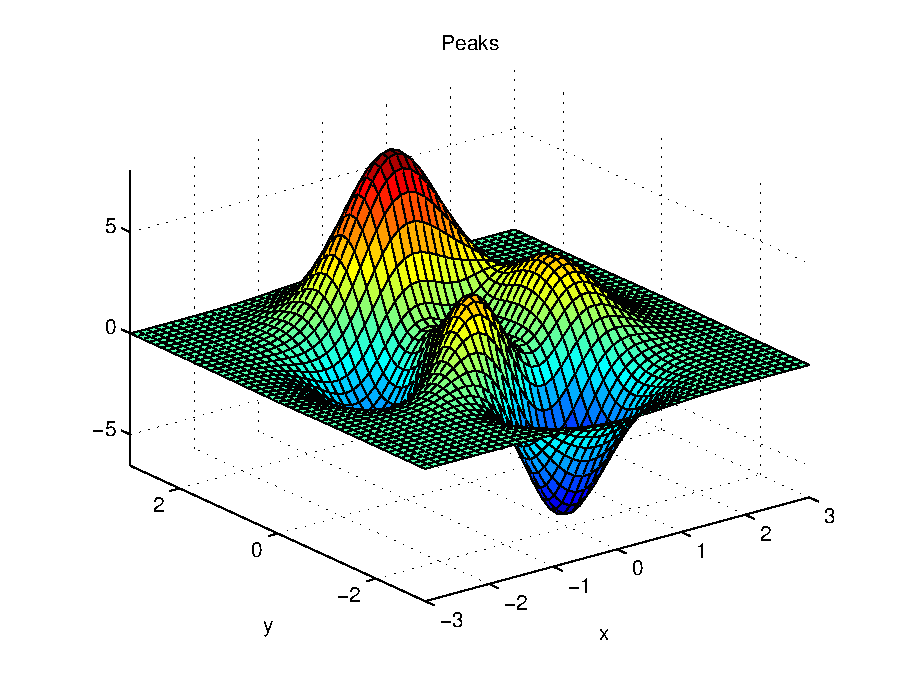
\includegraphics[width=4in]{egpic.eps}
\caption{图的名字}
\end{center}
本图来源:国家信息中心报告,《2005-2006年汽车市场分析与预测》,第24页。
\end{figure}
jwc.uibe.edu.cn里Word模版的图没找到\footnote{这又是一个脚注}。
\subsection{插表}
\begin{table}[H]
  \centering 
  \caption{中国汽车普及地区分类}\label{ }
  \vspace{.5em}
  \begin{tabular}{|c|c|c|c|}
\hline
   & 一类地区 &  二类地区\\\hline
 城市名  & 北京、上海 & 江苏、浙江、山东、广东 \\\hline
  人口总量(亿) & 0.32 & 2.96(为一类地区的9.2倍) \\\hline
  GDP总量(万亿元) & 1.17 & 5.83(为一类地区的5倍) \\\hline
人均GDP(US\$) & 4596 & 2480 \\\hline
小型微型客车保有量(万辆) & 200.7 & 488.57 \\\hline
\end{tabular}

\vspace{.5em}
本表来源:国家信息中心报告,《2005-2006年汽车市场分析与预测》,第23页。
\end{table}
根据jwc的规定表标题一定表上边但是图标题一定表下面。
\subsection{插入公式}
根据瓦尔拉斯定律
\begin{eqnarray}
\sum_{i=1}^N P_iQ_i^d & = & \sum_{i=1}^N P_iQ_i^s 
\end{eqnarray}
\section{实证研究}
\subsection{计量模型}
本文计量模型如下。
\begin{eqnarray}
\ln(\mathrm{Vx}_{rst}) = \beta\ln(\mathrm{FDI}_{srt}) + \bm\Phi_{rs} + \bm\Psi_t+\epsilon_{rst}\hspace{1cm}(\mathrm{x} = 1,2,3,4)
\end{eqnarray}
回归表格范式如下(建议用STATA的outreg2命令或者R语言的stargazer package导出\TeX 版)
\begin{table}[H] \centering 
\caption{回归结果}
\vspace{0.5em}
  \small
\begin{tabular}{@{\extracolsep{5pt}}lcccccc} 
\\[-3ex]\hline 
\hline \\[-3ex] 
\\[-4ex] & \multicolumn{3}{c}{log(v3)} & \multicolumn{3}{c}{log(v4)} \\ 
\\[-4ex] & (9) & (10) & (11)  & (13) & (14) & (15) \\ 
\hline \\[-1.8ex] 
 log(FDI$_{t}$) & 0.0026$^{***}$ & 0.0028$^{***}$ & 0.0028$^{***}$ & 0.0012$^{**}$ & 0.0013$^{**}$ & 0.0014$^{***}$  \\ 
  & (0.0010) & (0.0010) & (0.0010)  & (0.0005) & (0.0005) & (0.0005)  \\ 
  & & & & &   \\ 
 log(FDI$_{t-2}$) &  & 0.0034$^{***}$ & 0.0036$^{***}$ &  & 0.0026$^{***}$ & 0.0027$^{***}$ \\ 
  &  & (0.0010)  & (0.0010) &  & (0.0006) & (0.0006)  \\ 
  & & & & &   \\ 
 log(FDI$_{t-4}$) &  &  & 0.0005 &  &  & 0.0015$^{**}$  \\ 
  &  &  & (0.0011)  &  &  & (0.0006)  \\ 
  & & & & &   \\ 
      \hline
  Year FE&Yes&Yes&Yes&Yes&Yes&Yes\\
  Country-Pair FE&Yes&Yes&Yes&Yes&Yes&Yes\\
    \hline\\[-1.8ex]
Observations & 25,350 & 25,350 & 25,350  & 25,350 & 25,350 & 25,350\\ 
R$^{2}$ & 0.0003 & 0.0009 & 0.0009  & 0.0002 & 0.0012 & 0.0015  \\ 
\hline \\[-1.8ex] 
\textit{Notes:} & \multicolumn{6}{l}{$^{***}$Significant at the 1 percent level.} \\ 
 & \multicolumn{6}{l}{$^{**}$Significant at the 5 percent level.} \\ 
 & \multicolumn{6}{l}{$^{*}$Significant at the 10 percent level.} \\ 
\end{tabular} 
\label{hgjg2} 
\end{table} 
根据表\ref{hgjg2}的回归结果我们可以看出,*输入你的结论*
\section{如何引用}
推荐使用biblatex来整理(因为只有biblatex可以实现文中citation是author-year引用但结尾的参考文献中却是标号引用、以及中文英文文献分开生成。是的jwc就是这么bt),这个模版使用的Author-year形式的引用格式。\\
例1:这是一个引用\citep{autor2016china}。

同时也可以将作者从括号中拿出,改成Author (year)的形式。\\
例2:\citet{a}曾提出过……

每篇文献的.bib文件都可以在谷歌学术、百度学术、必应学术批量下载,很方便。引用的时候只需要\verb"\citep{handle}"、\verb"\citet{handle}"或者\verb"\cite{handle}"即可。详细可参加natbib的引用方法。

中文引用与英文无异\\
例3:这是一个中文文献引用\citep{stephen2014}。

\addcontentsline{toc}{subsection}{}
\newpage
\addcontentsline{toc}{section}{参考文献}
\section*{参考文献}
\titleformat{\section}
{\zihao{-4}\bfseries}
{\thesubsection}
{0pt}
{}
\titlespacing*{\section}{0pt}{1ex plus 1ex minus .3ex}{0pt}

\printbibliography[title=一、中文部分, keyword=zh, resetnumbers = 1]
\printbibliography[title=二、英文部分, keyword=en, resetnumbers = 1]


\addcontentsline{toc}{subsection}{}
\newpage
\begin{appendix}
\titleformat{\section}
{\zihao{-3}\bfseries}
{\thesubsection}
{0pt}
{}
\section*{附录\ \ \ \ 外文译文两篇}
\addcontentsline{toc}{section}{附录\ \ \ \ 外文文献译文两篇}
\begin{center}
\vspace{3ex}
\zihao{-3}\textbf{译文一}\ \ \ \ \textbf{测算全球价值链参与度和全球经济周期}\\
\vspace{1.5ex}
Zhi Wang\\
Shang-Jin Wei\\
Xinding Yu\\
Kunfu Zhu\\
\vspace{1.5ex}
\zihao{-4}孙晔 \quad 译\\
\vspace{1.5ex}
\end{center}
……在不失的一般性的情况下, 让我们考虑一个拥有 $G$ 国和 $N$ 部门的世界经济。其经济结构由表1中的以下国家间投入产出模型表示:

\begin{center}
(表 1)
\end{center}

其中 $Z^{sr}$ 是一个$N×N$矩阵,表示在国家 $s$ 中产生并用于国家 $r$ 的中间投入;$Y^{sr}$ 是一个$N ×1$向量,表示在国家生产的最终产品 $s$ 和在国家 $r$ 消费;$X^s$ 也是一个 $Nx1$ 向量,表示国家 $s$的总产出/总投入;$VA^s$是 表示在国家 $s$ 美元的直接增值的 $1×N $ 向量。在此 ICIO 模型中, 输入系数矩阵可以定义为 $A = Z\hat{X} ^ {-1} $, 其中 $ \hat{x} $ 表示在其对角线中输出向量 $X $ 的对角线矩阵。值加能系数向量可以定义为 $V = V \hat {X} ^ {-1}$。总产出$X$可分为中间产品和最终产品,即$AX + Y = X$。重新整理公式后,我们可以推导出经典的里昂惕夫方程,$X = BY$。其中 $B = (I-A) ^ {-1} $即位众所周知的(全局)Leontief 逆矩阵。
\newpage
\section*{附原文}
\begin{center}
\vspace{3ex}
\zihao{-3}\textbf{
Measures of Paticipation in Global Value Chains and Global Business Cycles}\\
\vspace{1ex}
Zhi Wang\\
Shang-Jin Wei\\
Xinding Yu\\
Kunfu Zhu\\
\end{center}
...Without loss generality, let us consider a world economy with G countries and N sectors. Its economic structure is represented by the following Inter-Country Input- Output (ICIO) model in Table 1:

\begin{center}
(Table 1)
\end{center}

where $Z^{sr}$ is an $N×N$ matrix of intermediate input flows that are produced in country $s$ and used in country $r$; $Y^{sr}$ is an $N×1$ vector giving final products produced in country $s$ and consumed in country $r$; $X^s$ is also an $N×1$ vector giving gross outputs in country $s$; and $VA^s$ denotes a $1×N$ vector of direct value added in country $s$. In this ICIO model, the input coefficient matrix can be defined as $A = Z\hat{X}^{-1}$, where $\hat{X}$ denotes a diagonal matrix with the output vector $X$ in its diagonal. The value added coefficient vector can be defined as $V = Va\hat{X}^{-1}$
. Gross outputs $X$ can be split into intermediate and final products, $AX + Y = X$
. Rearranging terms, we can reach the classical Leontief (1936) equation, $X = BY$,
where $B = (I-A)^{-1}$is the well-known (global) Leontief inverse matrix.
\newpage
\begin{center}
\vspace{3ex}
\zihao{-3}\textbf{译文二}\quad\textbf{全球价值链中的潜在和实际FDI溢出效应 - 外国投资者特征,吸收能力和传导渠道的作用}\\
\vspace{1.5ex}
Deborah Winkler\\
\vspace{1.5ex}
\zihao{-4}孙晔 \quad 译\\
\vspace{1.5ex}
\end{center}
……利用新收集的关于智利,加纳,肯尼亚,莱索托,莫桑比克,斯威士兰和越南直接供应商 - 多国联系的调查数据,本文评估了外国投资者在整体业绩,与当地经济的联系方面是否与国内生产者不同,和供应商的协助都会影响企业产生生产力溢出的潜力。除服装外,我们样本中的公司涵盖两个自然资源密集型行业,即农业综合企业和采矿业。我们发现外国投资者在销售额,公司规模,生产力,出口行为和直接出口份额方面均优于国内生产商。虽然与国内企业相比,这意味着更高的知识和生产率溢出潜力,但外国投资者在使用国内投入和工人方面与当地经济的联系较少。然而,调查结果还表明,某些服务投入,即技术服务和运输,安全,清洁,餐饮和其他服务,显示出更高的联系潜力。还有一些证据表明,外国公司向当地供应商提供的援助较少。较少的联系和供应商援助都可以限制外国直接投资的积极影响。

\newpage
\section*{附原文}
\begin{center}
\vspace{3ex}
\zihao{-3}\textbf{
Potential and Actual FDI Spillovers in Global Value Chains - The Role of Foreign Investor Characteristics, Absorptive Capacity and Transmission Channels}\\
\vspace{1ex}
Deborah Winkler\\
\end{center}
...Using newly collected survey data on direct supplier-multinational linkages in Chile, Ghana, Kenya, Lesotho, Mozambique, Swaziland, and Vietnam, this paper evaluated whether foreign investors differ from domestic producers in terms of their overall performance, linkages with the local economy, and supplier assistance which all influence the firms’ potential to generate productivity spillovers. Besides apparel, the firms in our sample cover two natural resources- intensive industries, namely agribusiness and mining. We found that foreign investors outperform domestic producers in terms of sales, firm size, productivity, exporting behavior, and direct export share. While this would imply a higher knowledge and productivity spillover potential compared to domestic firms, foreign investors have fewer linkages with the local economy in terms of using domestic inputs and workers. However, the findings also show that certain service inputs, namely technical services and transport, security, cleaning, catering, and other services, show a higher potential for linkages. There is also some evidence that foreign firms offer less assistance to local suppliers. Fewer linkages and supplier assistance both can limit the positive impact from FDI.
\end{appendix}
\newpage
\addcontentsline{toc}{subsection}{}
\titleformat{\section}
{\zihao{-3}\bfseries\centering}
{\thesection、}
{0pt}
{}
\titlespacing*{\section}{0pt}{1ex plus 1ex minus .3ex}{2ex}
\section*{致谢}
\addcontentsline{toc}{section}{致谢}
笔者承*键入老师姓名*老师悉心指导……
\vspace{2em}
\begin{flushright}
姓名\ \ \ \ \ \ \ \ \ \ \ \ \ \ \ \ \ \\
\hspace{2em}年\hspace{2em}月
\end{flushright}


\end{document} 